\documentclass{article}

\usepackage{geometry}[margin = 0.5in]
\usepackage{graphicx}

\begin{document}

\section{Phase portrait of the regularized system with varying epsilon values}

\begin{figure}[bht] \begin{center}
    \begin{tabular}{c c}
    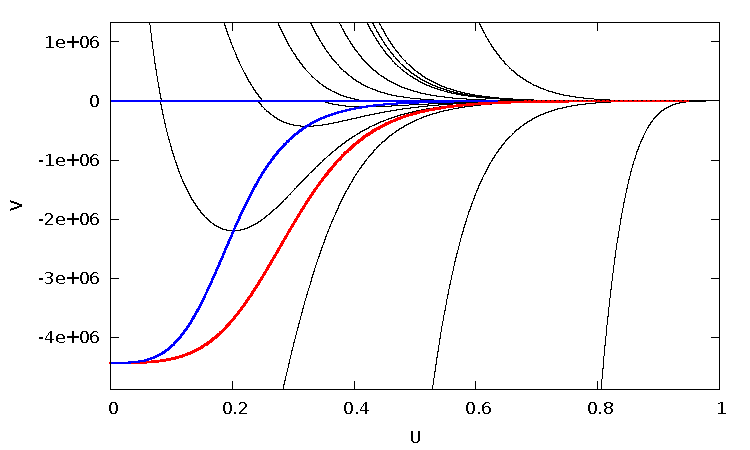
\includegraphics[scale = 0.5]{regPhasePlane_epsilon10e-1.pdf} &
    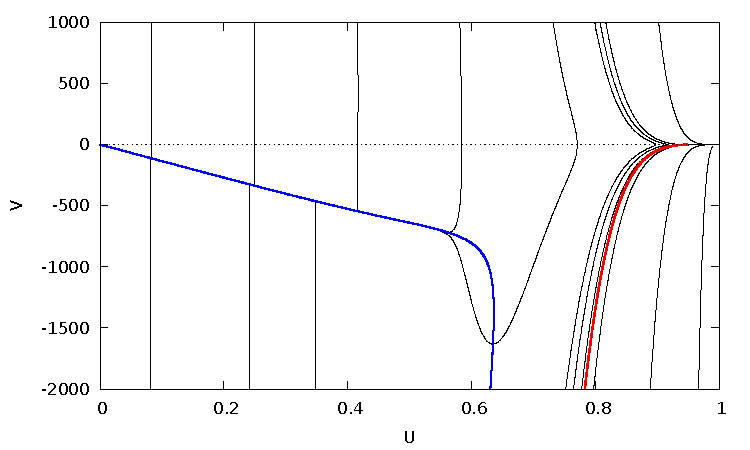
\includegraphics[scale = 0.5]{regPhasePlaneZoomed_epsilon10e-1.pdf} \\
    (a) & (b)\\
    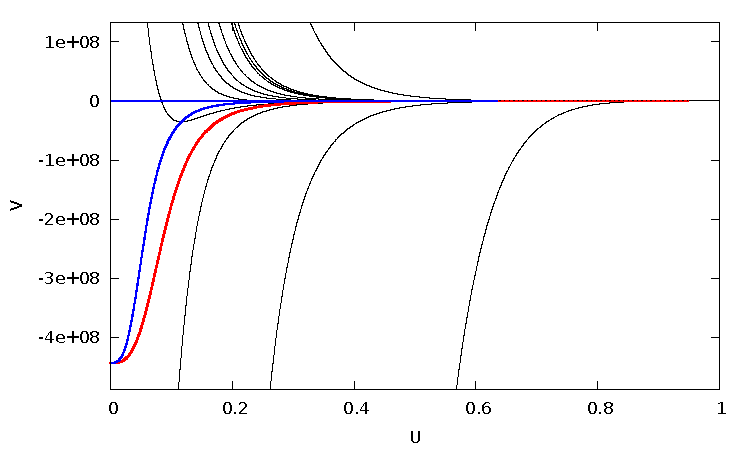
\includegraphics[scale = 0.5]{regPhasePlane_epsilon10e-3.pdf} &
    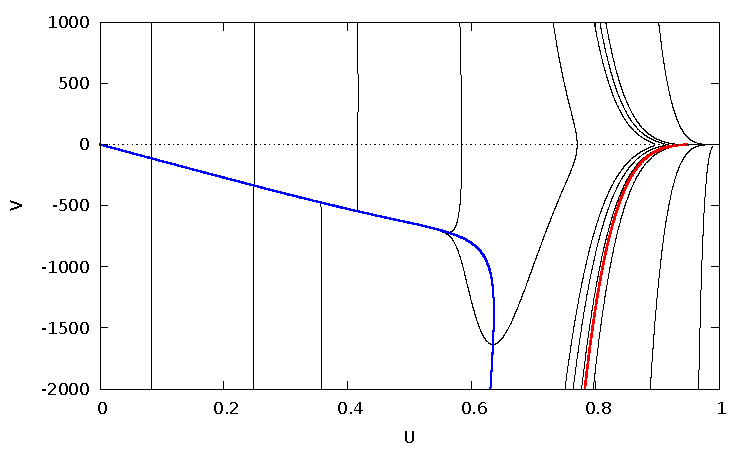
\includegraphics[scale = 0.5]{regPhasePlaneZoomed_epsilon10e-3.pdf} \\
    (c) & (d)\\
    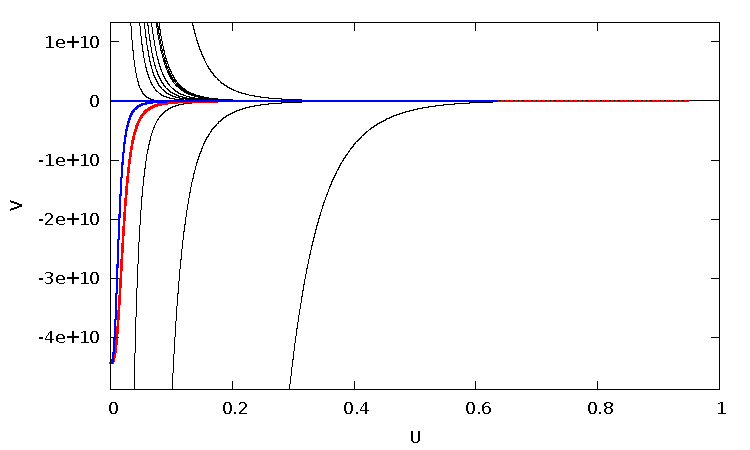
\includegraphics[scale = 0.5]{regPhasePlane_epsilon10e-5.pdf} &
    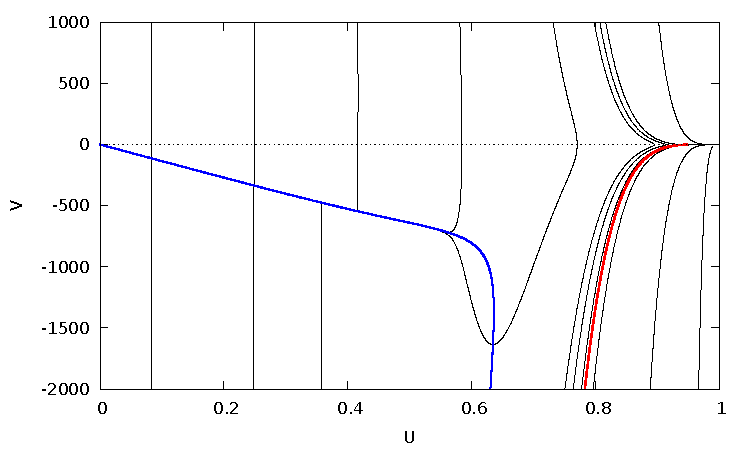
\includegraphics[scale = 0.5]{regPhasePlaneZoomed_epsilon10e-5.pdf} \\
    (e) & (f)   
    \end{tabular}
    
    \caption{Phase portrait of the regularized system with:
    (a) $\epsilon = 10^{-1}$, 
    (c) $\epsilon = 10^{-3}$, 
    (e) $\epsilon = 10^{-5}$. 
    \\(b), (d), and (f) are the cooresponding phase portraits zoomed onto the U-axis.
    \\ Note: the red line represents the traveling wave and the blue line is the V-Nullcline.}
\end{center} \end{figure}



\end{document}




